\documentclass{article}


\usepackage[margin=0.6in]{geometry}
\usepackage{amssymb, amsmath, amsfonts}
\usepackage{mathtools}
\usepackage{physics}
\usepackage{enumerate}
\usepackage{array}
\usepackage{tikz}
\usepackage{pgfplots}
\newcommand{\Rl}{\mathbb{R}}
\newcommand{\E}{\varepsilon}
\newcommand{\f}[3]{#1\ :\ #2 \rightarrow #3}

\title{MAT 228A Notes}
\author{Sam Fleischer}
\date{September 27, 2016}

\begin{document}
    \maketitle

    \section{Solving the Poisson Equation using Fourier Series}
        In 1-D, suppose $u_{xx} = f$ on $(0,1)$ with $u(0) = u(1) = 0$.  Note that if $f = -(n\pi)^2\sin(n\pi x)$ then the solution is $u = \sin(n\pi x)$ by observation.  Reframe the problem as $L u = f$ with $L = \dfrac{\partial^2}{\partial x^2}$.  Then with $u_n \coloneqq \sin (n\pi x)$, we have
        \begin{align}
            Lu_n = -(n\pi)^2 u_n
        \end{align}
        and thus $u_n$ is an eigenfunction of $L$ with eigenvalue $-(n\pi)^2$.  We can show they are orthogonal in $L^2(0,1)$ by
        \begin{align}
            \langle\sin(n\pi x),\sin(m\pi x)\rangle_{L^2(0,1)} = \int_0^1 \sin(n\pi x)\sin(m\pi x)\dd x = \begin{cases}
                \frac{1}{2} & \text{ if } n \neq m \\
                0 & \text{ else }
            \end{cases}.
        \end{align}
        It also turns out these eigenfunctions form a complete set in $L^2$, that is $\{u_n\}_{n=1}^\infty$ is a basis.  Thus, for a given $f \in L^2(0,1)$, there are coefficients $a_n$ such that
        \begin{align}
            f(x) = \sum_{n=1}^\infty a_n u_n(x)
        \end{align}
        where the convergence is in $\norm{\cdot}_{L^2(0,1)}$.  The solution $u$ of $Lu = f$ can also be written as a linear combination of $u_n$,
        \begin{align}
            u(x) = \sum_{n=1}^\infty \beta_n u_n(x)
        \end{align}
        We can use orthogonality of $u_n$ to explicitly compute $a_n$, and we obtain
        \begin{align}
            a_n = 2\langle f(x),u_n(x)\rangle_{L^2(0,1)}
        \end{align}
        Finally, we have
        \begin{align}
            L\qty[\sum \beta_n u_n(x)] = \sum a_n u_n(x),
        \end{align}
        and we exploit orthogonality again, taking an inner product of both sides with $u_m$, and we obtain
        \begin{align}
            \beta_n = -\frac{a_n}{(n\pi)^2} \qquad \text{ for } n = 1, 2, \dots.
        \end{align}

        In 2-D, it is the same basic idea.  We have $\laplacian u = u_{xx} + u_{yy} = f$ on $(0,1) \times (0,1)$ with $u(x,y) = 0$ on the boundary.  The eigenfunctions are given by
        \begin{align}
            u_{n,m}(x) = \sin(n\pi x)\sin(m\pi y) \qquad \text{ for } n,m = 1, 2, \dots
        \end{align}
        with eigenvalues $\lambda_{n,m} = -(n^2 + m^2)\pi^2$.  The remaining calculations of the general solution to $\laplacian u = f$ for any $f \in L^2((0,1)^2)$ are similar to the solution in 1-D.

        \section{Methods of Solving PDEs Numerically}
            \subsection{Finite Differences}
                Given a PDE, a domain $\Omega$, and boundary conditions, we take the following steps:
                \begin{enumerate}[\ \ 1)]
                    \item Discretize the Domain $\Omega$, that is, represent $\Omega$ by a set of points.  For example, draw a grid and the points are at the intersections and at the boundary.
                    \item Represent functions by values at those points.
                    \item Use discrete values to approximate derivatives using algebraic formulas
                \end{enumerate}
                The result, assuming the PDE is linear, is an algebraic equation of the form
                \begin{align}
                    A\underline(u) = \underline{b}.
                \end{align}
            \subsection{Finite Elements}
                Reformulate the problem as a variational problem.  Rather than solving $\laplacian u = f$, define the functional $F$ by
                \begin{align}
                    F(u) \coloneqq \int_\Omega \frac{1}{2}\grad u \cdot \grad u + u f \dd x.
                \end{align}
                The minimizer of $F$ also solves $\laplacian u = f$ (using the Euler-Lagrange equation).  So we want to find $u \in S$ to minimize $F$ where $S$ is the space of ``admissible'' functions.

                Now let's discretize the function space, i.e.~choose a subset of the basis elements of $S$ to represent $S$.  Define this subset $S_h$, where $\dim S_h = N < \infty$.  Then for any $u_h \in S_h$,
                \begin{align}
                    u_h(x) = \sum_{k=1}^N a_k \phi_k(x)
                \end{align}
                A good basis $\{\phi_k\}_{k=1}^N$ for $S_h$ are tent functions with small overlap, for example,
                \begin{center}
                    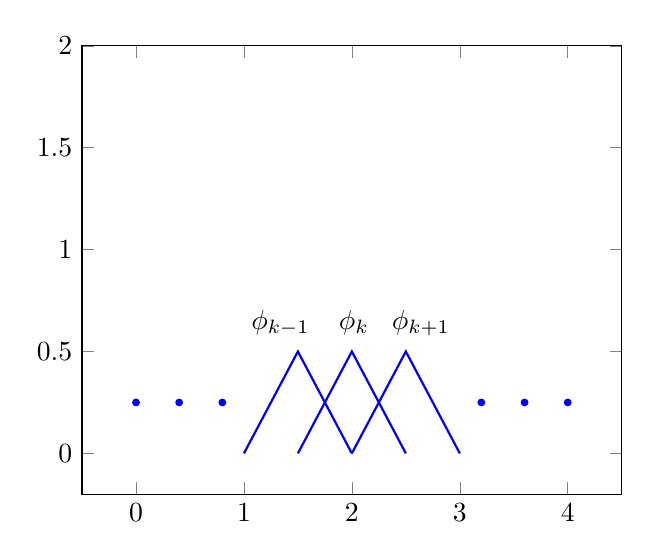
\begin{tikzpicture}
                        \begin{axis}[ymax=2,xmin=-0.5,xmax=4.5]
                            \node[blue,circle,fill,inner sep=1pt] at (axis cs:0,0.25) {};
                            \node[blue,circle,fill,inner sep=1pt] at (axis cs:0.4,0.25) {};
                            \node[blue,circle,fill,inner sep=1pt] at (axis cs:0.8,0.25) {};
                            \addplot[blue,thick] coordinates {(1,0) (1.5,0.5) (2,0)};
                            \node at (axis cs:1.7,0.75) [anchor=north east] {$\phi_{k-1}$};
                            \addplot[blue,thick] coordinates {(1.5,0) (2,0.5) (2.5,0)};
                            \node at (axis cs:2.25,0.75) [anchor=north east] {$\phi_{k}$};
                            \addplot[blue,thick] coordinates {(2,0) (2.5,0.5) (3,0)};
                            \node at (axis cs:3,0.75) [anchor=north east] {$\phi_{k+1}$};
                            \node[blue,circle,fill,inner sep=1pt] at (axis cs:3.2,0.25) {};
                            \node[blue,circle,fill,inner sep=1pt] at (axis cs:3.6,0.25) {};
                            \node[blue,circle,fill,inner sep=1pt] at (axis cs:4,0.25) {};
                        \end{axis}
                    \end{tikzpicture}
                \end{center}
                It turns out $S_h$ is the space of ``connect-the-dot'' functions (piecewise linear functions).  Then we can approximate a function $u \in L^2$ by its closest representation using the basis $\{\phi_k\}_{k=1}^N$, i.e.
                \begin{align}
                    u(x) \approx u_h(x) \coloneqq \sum_{k=1}^N a_k \phi_k(x).
                \end{align}
                The projection theorem tells us there are unique $\{a_k\}$ such that $\norm{u - u_h}_{L^2}$ is minimized.
                
                Anyway, this looks a lot like finite differences, but is philosophically different: the function space is discretized, but not the domain.

                Finally, we can solve a minimization problem on $S_h$.  What does $F(u_h)$ look like?
                \begin{align}
                    F(u_h) = \frac{1}{2}\sum_{i,j=1}^N A_{i,j}a_i a_j + \sum_{i=1}^N b_i a_i
                \end{align}
                where
                \begin{align}
                    A_{i,j} = \int_\Omega \grad \phi_i \cdot \grad \phi_j \dd x \qquad \text{and} \qquad b_i = \int_\Omega f(x) \phi_i(x) \dd x
                \end{align}
                and $a_i$ are unknown.  To minimize this expression with respect to $\{a_1, \dots, a_N\}$, we take partial derivatives with respect to each $a_i$, i.e. $\grad[a_1, \dots, a_N]$, and set it equal to zero.  However,
                \begin{align}
                    \grad F = 0 \implies A \underline{a} = \underline{b},
                \end{align}
                which is a linear system.  It turns out that for very simple problems, this is identical to the linear system we acheive using finite differences.

                Note that we chose a locally-supported since this gives rise to a sparse matrix $A$, which is easier to solve than arbitrary systems.

            \subsection{Spectral Methods}
                We can use a representation of $u$, i.e.
                \begin{align}
                    u_h(x) = \sum_{k=1}^N a_k \phi_k(x)
                \end{align}
                where $\phi_k$ are known functions (not limiting ourselves to locally-supported $\phi_k$), for example, take $\phi_k = \sin k\pi x$.  From here,
                \begin{enumerate}[\ \ 1)]
                    \item Solve the variational problem (but $A$ is not sparse - compuationally expensive)
                    \item For a set of points $\left\{x_1,\dots, x_N\right\}$ in the domain $\Omega$, solve $\laplacian u x_i = f(x_i)$.  That is, actually solve the PDE on the grid points (spectral collocation, which is a generalization of the finite differences method).
                \end{enumerate}
                Thus, again, we have
                \begin{align}
                    \sum_{i,j=1}^N a_j \phi_j(x_i) \qquad \text{for i,j = 1, 2, \dots N.}
                \end{align}
                And once again we get a linear system:
                \begin{align}
                    A_{ij} = \phi_j^{''}(x_i),
                \end{align}
                The main problems of this method are
                \begin{itemize}
                    \item In general, the matrix $A$ is dense, not sparse
                \end{itemize}

\end{document}
